% http://blog.jakob-wankel.de/2017/01/25/drawing-a-mechanical-system-with-tikz-in-latex/
\documentclass[border=15pt]{standalone}

\usepackage{tikz}
\usetikzlibrary{calc,patterns,decorations.pathmorphing,decorations.markings}


\begin{document}

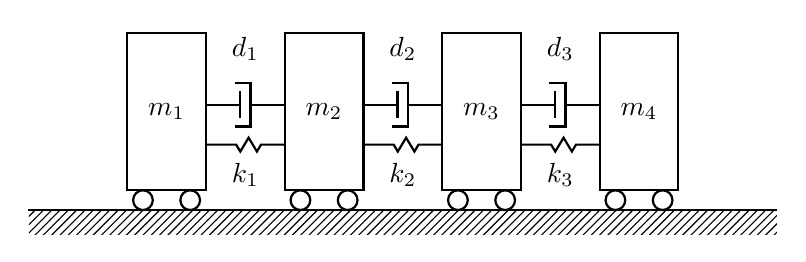
\begin{tikzpicture}
	\tikzstyle{spring}=[thick,decorate,decoration={zigzag,pre length=0.3cm,post length=0.3cm,segment length=6}]
	\tikzstyle{damper}=[thick,decoration={markings,  
		mark connection node=dmp,
		mark=at position 0.5 with 
		{
			\node (dmp) [thick,inner sep=0pt,transform shape,rotate=-90,minimum width=15pt,minimum height=3pt,draw=none] {};
			\draw [thick] ($(dmp.north east)+(2pt,0)$) -- (dmp.south east) -- (dmp.south west) -- ($(dmp.north west)+(2pt,0)$);
			\draw [thick] ($(dmp.north)+(0,-5pt)$) -- ($(dmp.north)+(0,5pt)$);
		}
	}, decorate]
	\tikzstyle{ground}=[fill,pattern=north east lines,draw=none,minimum width=0.75cm,minimum height=0.3cm]

	\node (M) [draw,outer sep=0pt,thick,minimum width=1cm, minimum height=2cm] {$m_1$};
	\node (M2) [draw,outer sep=0pt,thick,minimum width=1cm, minimum height=2cm] at (2,0) {$m_2$};
	\node (M3) [draw,outer sep=0pt,thick,minimum width=1cm, minimum height=2cm] at (4,0) {$m_3$};
	\node (M4) [draw,outer sep=0pt,thick,minimum width=1cm, minimum height=2cm] at (6,0) {$m_4$};

	\node (ground) [ground,anchor=north,xshift=3cm,yshift=-0.25cm,minimum width=9.5cm] at (M.south) {};

	\draw (ground.north east) -- (ground.north west);
	\draw [thick] (M.south west) ++ (0.2cm,-0.125cm) circle (0.125cm)  (M.south east) ++ (-0.2cm,-0.125cm) circle (0.125cm);
	\draw [thick] (M2.south west) ++ (0.2cm,-0.125cm) circle (0.125cm)  (M2.south east) ++ (-0.2cm,-0.125cm) circle (0.125cm);
	\draw [thick] (M3.south west) ++ (0.2cm,-0.125cm) circle (0.125cm)  (M3.south east) ++ (-0.2cm,-0.125cm) circle (0.125cm);
	\draw [thick] (M4.south west) ++ (0.2cm,-0.125cm) circle (0.125cm)  (M4.south east) ++ (-0.2cm,-0.125cm) circle (0.125cm);

	\draw [spring] (M2.220) -- ($(M.north east)!(M.220)!(M.south east)$);
	\draw [spring] (M3.220) -- ($(M2.north east)!(M2.220)!(M2.south east)$);
	\draw [spring] (M4.220) -- ($(M3.north east)!(M3.220)!(M3.south east)$);

	\draw [damper] (M2.170) -- ($(M.north east)!(M2.170)!(M.south east)$);
	\draw [damper] (M3.170) -- ($(M2.north east)!(M3.170)!(M2.south east)$);
	\draw [damper] (M4.170) -- ($(M3.north east)!(M4.170)!(M3.south east)$);

	\node at (1,.8) {$d_1$};
	\node at (3,.8) {$d_2$};
	\node at (5,.8) {$d_3$};

	\node at (1,-.8) {$k_1$};
	\node at (3,-.8) {$k_2$};
	\node at (5,-.8) {$k_3$};

\end{tikzpicture}

\end{document}
